\documentclass[11pt]{report}

\usepackage{polski}
\usepackage[utf8]{inputenc}
\usepackage{geometry}
\newgeometry{left=0.8in,right=0.8in,top=1in,bottom=1in}
\usepackage{graphicx}
\usepackage{subcaption}
\usepackage{float}
\usepackage{amssymb}
\usepackage{flexisym}
\usepackage{listings}
\renewcommand{\thesection}{\arabic{section}.}
\renewcommand{\thesubsection}{\arabic{section}.\arabic{subsection}.}
\usepackage{makecell}
\usepackage[hidelinks]{hyperref}
\usepackage[dvipsnames]{xcolor}
\usepackage[nottoc]{tocbibind}
\usepackage{fancyhdr}
\pagestyle{fancy}

\graphicspath{{images/}}

\lhead{}
\rhead{Metody ewolucyjne i uczenie się maszyn}

\begin{document}
\thispagestyle{empty}

\begin{flushright}
\large{Warszawa, \today}
\end{flushright}

\vspace{5 cm}

\begin{center}
\LARGE{\textbf{Metody ewolucyjne i uczenie się maszyn}}

\vspace{5 mm}

\Large{\textbf{Projekt 2}}

\Large{\textbf{Dokumentacja końcowa}}

\vspace{5 mm}

\Large{\textbf{Na jednym z benchmarków dot. modelowania szeregów czasowych (np. NN3 lub M3) porównać metodę XGBoost z modelem liniowym.}}
\end{center}

\vspace{3 cm}

\begin{flushright}
\large{Prowadzący:}

\large{dr inż. Paweł Zawistowski}
\end{flushright}

\vspace{1 cm}

\begin{flushright}
\large{Wykonali:}

\large{Michał Kruszewski, Łukasz Blaszka}
\end{flushright}

\newpage

\tableofcontents
\newpage

\section{Cel}
Celem projektu było praktyczne poznanie dowolnie wybranego modelu liniowego oraz metody XGBoost, stosowanych do modelowania szeregów czasowych.
Jako model liniowy wybrany został popularny model ARIMA (\textit{ang. AutoRegressive Integrated Moving Average}).
Realizacja celu oparta została na porównaniu obu metod na benchmark'u NN3.

\section{Założenia}
W specyfikacji wstępnej projektu znalazły się następujące założenia:

\begin{itemize}
\item Zadanie rozwiązane miało zostać w języku \textit{R}.

\item Jako benchmark testowy wybrany został nowszy benchmark NN3.
Zawiera on mniej szeregów czasowych niż benchmark M3 (111 vs 3003), dlatego lepiej nadaje się do celów dydaktycznych (subiektywna ocena osób realizujących projekt).

\item Jako model liniowy wybrany miał zostać popularny model ARIMA (\textit{ang. AutoRegressive Integrated Moving Average}), uznawany za jedną z opcji do modelowania szeregów niestacjonarnych.

\item W celu dopasowania najlepszego modelu ARIMA wykorzystana miała zostać metoda \textit{auto.arima} pochodząca z pakietu \textit{forecast}.

\item W celu predykcji metodą XGBoost wykorzystana miała zostać biblioteka \textit{XGBoost} (\url{https://github.com/dmlc/xgboost}).

\item Ze względu na brak jakiegokolwiek doświadczenia z metodą XGBoost, oraz liczbę jej parametrów, sposób optymalizacji określony miał zostać na etapie implementacji.
\end{itemize}

\section{Krótki wstęp teoretyczny}

\subsection{ARIMA}
Model ARIMA jest rozszerzeniem modelu ARMA, który poddawany jest różnicowaniu w celu usunięcia trendu.
Model ARMA(p,q) dla stacjonarnego szeregu czasowego $z_t$ ma postać:
\begin{equation}
    z_t = \phi_1 z_{t-1} + ... + \phi_p z_{t-p} + w_t + \psi_1 w_{t-1} + ... + \psi_q w_{t-q}
\end{equation}
gdzie $z_t$ jest szeregiem stacjonarnym o zerowej średniej, $\phi_i,\psi_i \in \mathbb{R} (\phi_p \neq 0, \psi_q \neq 0)$, a $w_i \sim N(0, \sigma^2)$.

Model ARMA jest połączeniem dwóch modeli:
\begin{itemize}
\item Model AR(p) - proces autoregresyjny $p$ rzędu określa wpływ $p$ poprzednich obserwacji na wartość obecną $z_t$.
Przy wyliczaniu modelu AR poszukiwane są wartości $(\phi_1, ..., \phi_p)$ by spełnić równanie\cite{armia_s_zajac}:
\begin{equation}
    z_t = c + \phi_1 z_{t-1} + \phi_2 z_{t-2} + ... + \phi_p z_{t-p}+w
\end{equation}


\item Model MA(q) - średnia ruchoma $q$ rzędu opisuje zależność obserwacji $z_t$ od aktualnego zakłócenia $w_t$ oraz $q$ poprzednich.  Poszukiwane są wartości $(\psi_1, ..., \psi_q)$ przy znanych wartościach zakłóceń $(w_1, ..., w_t)$. Wzór modelu MA\cite{armia_s_zajac}: 
\begin{equation}
    z_t = c + \psi_1 w_{t-1} + \psi_2 w_{t-2} + ... + \psi_q w_{t-q} + w_t
\end{equation}
\end{itemize}

Model ARIMA do usuwania trendu wykonuje operację różnicowania szerego gdzie d to opóźnienie (lag). Wzór różnicowania szeregu\cite{armia_s_zajac}:
\begin{equation}
    z_{t}'=z_t-z_{t-d}
\end{equation}
Ostatecznie model ARIMA(p,d,q) ma postac\cite{armia_s_zajac}:
\begin{equation}
    z_t' = c + \phi_1 z_{t-1}' + ... + \phi_p z_{t-p}' + w_t + \psi_1 w_{t-1} + ... + \psi_q w_{t-q}
\end{equation}

Sezonowy model ARIMA(p,d,q)(P,D,Q)$_s$ jest stosowany dla szeregów w których występuje sezonowość. Model ma następującą postać:
\begin{equation}
( 1-\psi_1 B - ... \psi_p B^P )(1-\Psi_1B^S-\Psi_2 B^2s - \Psi_p B^{Ps})y'' = (1-\phi_1 B - ,.. - \phi_q B^q)(1-\Phi_1 B^s - \Phi_2 B^2s - \Phi_Q B^{Qs})\epsilon_t
\end{equation}
gdzie y’’ jest szeregiem różnicowanym D-krotnie z opóźnieniem s, a następnie d-krotnym z opóźnieniem 1, natomiast $B^ky_t=y_{t-k}$\cite{analiza_i_prognozy_szeregow_czasowych_quantup}.

\subsection{Funkcja auto.arima() w pakiecie R}
Pakiet R udostępnia funkcję auto.arima(). Zwraca ona model ARIMA lub sARIMA z parametrami które zostały określone na podstawie wartości AIC, AICc lub BIC.

AIC (\textit{ang. Akaike Information Criterion}), AICc (\textit{ang. Second-order Akaike Information Criterion}) i BIC (\textit{ang. Akaike Information Criterion}) są kryteriami doboru parametrów. Ich wyższa wartość świadczy o lepszym stanie modelu. Kryteria pozwalają na optymalny dobór parametrów dla uzyskania najlepszych rezultatów predykcji jednocześnie nie dopuścić do przeuczenia.

Funkcja auto.arima() umożliwia na uzyskanie modelu podając jedynie przebieg czasowy do szkolenia. 
Na proces automatycznego doboru można wpłynąć podając dodatkowe parametry przy wywołaniu. Poniżej wybrane parametry:
\begin{itemize}
\item Granice wartości parametrów dla modeli ARIMA(p,d,q) oraz sARIMA(p,d,q)(P,D,Q)$_s$
\item d - Kolejność pierwszego różnicowania, jeśli zostanie pominięty wartość zostanie określona na podstawie testu KPSS
\item D - Kolejność pierwszego różnicowania, jeśli zostanie pominięty wartość zostanie określona na podstawie testu OCSB
\item ic - wybór kryterium przy doborze parametrów (domyślnie AIC, BIC i AICc )
\item xreg - zewnętrzny wektor regresu
\item stationary - dla wartości TRUE to proces ograniczy się do modelu stacjonarnego
\item seasonal - dla wartości FALSE to proces ograniczy się do modelu nie sezonowego
\item allowdrift - dla wartości TRUE rozważane są modele z dryftem
\item allowmean - dla wartości TRUE rozważane są modele o niezerowej średniej.
\end{itemize}

\subsection{Metoda XGBoost}
Metoda XGBoost (\textit{Extreme Gradient Boosting}) wywodzi się z metody GBM (\textit{ang. Gradient Boosting Machine}).
Obie te metody opierają się o gradientowe wzmacnianie drzew (\textit{ang. gradient boosted trees}).
U ich podstaw znajduje się model zespołu drzew decyzyjnych (\textit{ang. decision tree ensembles}).
W zespole takim pojedyncze drzewo zazwyczaj słabo radzi sobie z klasyfikacją/regresją, dlatego do predykcji wykorzystywany jest cały zespół drzew.
Idea wzmacniania gradientowego polega na tworzeniu ciągu prostych drzew, z których każde kolejne jest zbudowane do predykcji reszt generowanych przez poprzednie.

Różnica w idei działania XGBoost a GDM jest niewielka.
XGBoost używa bardziej regularnej formalizacji modelu w celu kontroli przeuczenia (\textit{over-fitting}).
Dodatkowo XGBoost jest mocno zoptymalizowany w obszarach szybkości obliczeń oraz zużycia pamięci.

Podczas uczenia i przewidywania z wykorzystaniem modelu XGBoost kluczową rolę odgrywają 2 zbiory danych $X$ oraz $Y$.
Zbiór $X$ to tzw. zbiór atrybutów/cech (\textit{and. features}), natomiast zbiór $Y$ to tak zwany zbiór etykiet (\textit{ang. labels}).
W przypadku szeregów czasowych atrybutami/cechami mogą być wartości szeregu przesuniętego w czasie lub dowolne inne parametry wyznaczane na podstawie wartości szeregu czasowego.
Etykietami są wartości szeregów w poszczególnych chwilach czasowych.
Predykcja polega na wyznaczeniu wartości etykiety na podstawie odpowiadającej jej wartości atrybutów.

\section{Zbiór danych}
Liczba szeregów czasowych znajdujących się w benchmark'u NN3 wynosi 111.
Długość wektora testowego dla każdego z szeregów wynosi 18.
Zbiór danych jest zaczerpnięty z jednorodnej populacji empirycznych biznesowych szeregów czasowych.
Wśród danych dominują szeregi, które wydają się być mocno zaszumione (rys. \ref{fig:sfig1}, \ref{fig:sfig2}).
Znaleźć tam również można szeregi czasowe z wyraźnym trendem (rys. \ref{fig:sfig3}) lub wahaniami okresowymi (rys. \ref{fig:sfig4}).

\begin{figure}[H]
    \begin{subfigure}{.5\textwidth}
        \centering
        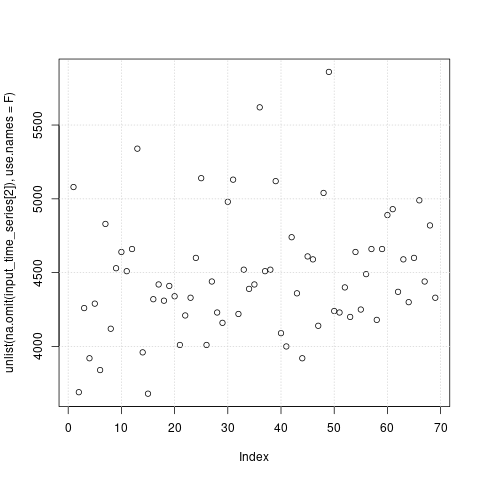
\includegraphics[width=.9\linewidth]{plot2.png}
        \caption{Dane zaszumione}
        \label{fig:sfig1}
    \end{subfigure}
    \begin{subfigure}{.5\textwidth}
        \centering
        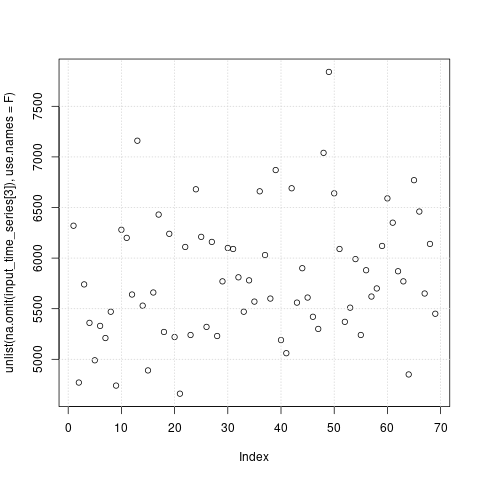
\includegraphics[width=.9\linewidth]{plot3.png}
        \caption{Dane zaszumione}
        \label{fig:sfig2}
    \end{subfigure}
    \begin{subfigure}{.5\textwidth}
        \centering
        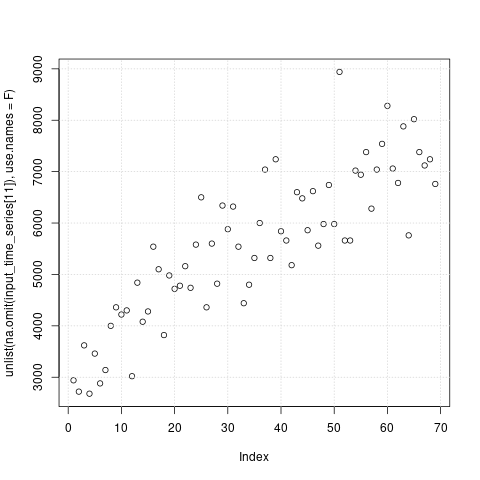
\includegraphics[width=.9\linewidth]{plot11.png}
        \caption{Trend}
        \label{fig:sfig3}
    \end{subfigure} \begin{subfigure}{.5\textwidth}
        \centering
        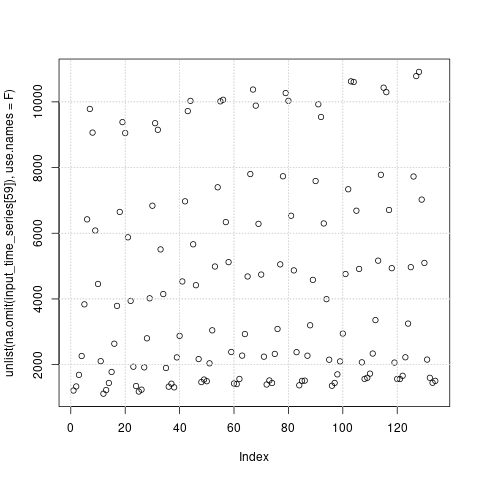
\includegraphics[width=.9\linewidth]{plot59.png}
        \caption{Wahania okresowe}
        \label{fig:sfig4}
    \end{subfigure}

    \caption{Przykładowe szeregi czasowe z benchmark'u NN3.}
    \label{fig:sample_time_series}
\end{figure}

Szeregi czasowe w benchmark'u NN3 są stosunkowo krótkie (min 68, max 144), a sam benchmark uznawany jest przez ekspertów z dzedziny modelowania szeregów czasowych jako dość ,,prosty''.

\section{Implementacja}

Szeregi czasowe z benchmark'u NN3 zostały znormalizowane do przedziału $<1:2>$ w celu umożliwienia porównywania błędów bezwzględnych.
Wadą normalizacji może być przeskalowanie większości z wartości szeregu do wąskiego przedziału w przypadku, kiedy w danych znajduje się co najmniej 1 mocno odstający punkt \cite{noauthor_standardization_nodate}.
Przesunięcie zakresu z przedziału $<0:1>$ do $<1:2>$ pozwala również na obliczanie błędów względnych bez obawy dzielenia przez 0.

Predykcja wartości odbywa się z krokiem o długości 1.
Oznacza to, iż przy predykcji wartości dla chwil czasowych $t+n$ wykorzystywane są rzeczywiste wartości szeregu z chwil czasowych wcześniejszych od $t+n$.

\subsection{ARIMA}
W predykcji z wykorzystaniem modelu ARIMA wsparto się funkcja auto.arima() która automatycznie dobiera parametry modelu dla 111 przebiegów czasowych.
Wykorzystano domyślnie definicje parametrów funkcji auto.arima() w zaufaniu, że pozwalają uzyskać optymalne wyniki dla nieokreślonej ilości przebiegów.

Predykcje z krokiem o długości 1 zrealizowano tworząc oddzielny model dla każdej wartości szeregu testowego. Szereg uczący w każdym kroku jest zwiększany o jedną wartość z szeregu testowego.
Do uzyskania przewidywanej wartości z wyliczonego modelu wykorzystaniu funkcję forecast. Parametr "h" określa dla ilu kroków ma zostać wyliczona przewidywana wartość.

Poniżej kod dokonuje predykcji z krokiem o długości 1 na podstawie wyliczonego modelu ARIMA'y dla N-tego przebiegu czasowego benchmark'u NN3:
\begin{lstlisting}[language=R]
learn_data_length = length( tmp_ts_learn )
for (j in 1:TEST_DATA_LENGTH) {
    ts_end = learn_data_length + j
    ts <- ts(tmp_ts[1:ts_end])
    arima_model = auto.arima(ts)
    arima_forecast_all = forecast(arima_model, h = 1)
    arima_forecast = as.data.frame(arima_forecast_all)$'Point Forecast'
    arima_forecast_oneAhead[j] = arima_forecast
}
\end{lstlisting}

\subsection{XGBoost}

Predykcja za pomocą metody XGBoost zrealizowana została na dwa sposoby, różniące się podejściem do wyboru atrybutów/cech wykorzystywanych do uczenia i przewidywania.

\subsubsection{XGBoost z subiektywnie wybranymi cechami}
Osoby realizujące projekt dokonały subiektywnego wyboru dwóch atrybutów.
Pierwszy z nich to miesiąc, z którego pochodzi dana wartość szeregu czasowego.
Drugi to tzw. wskaźnik siły względnej (\textit{ang. relative strength index}), określający siłę trendu.
Oparty jest on o średnią ruchomą \cite{noauthor_relative_2018}.
W projekcie obliczany jest z wykorzystaniem ważonej średniej ruchomej (\textit{ang. weighted moving average}).

\subsubsection{XGBoost na podstawie autokorelacji częściowej}
Metoda ta polegała na obliczaniu funkcji autokorelacji częściowej i wyznaczaniu na jej podstawie tzw. lagów, czyli wartości szeregu przesuniętych w czasie.
Wybrana została funkcji autokorelacji częściowej, a nie funkcja autokorelacji, ponieważ wydaje się być ona bardziej odpowiednia dla metod nieliniowych.
Autokorelacja częściowa dla lagu k jest korelacją, która usuwa efekt jakichkolwiek korelacji dla lagów krótszych niż k \cite{cowpertwait_introductory_2009}.
Ze względu na fakt, iż wszystkie szeregi czasowe z benchmark'u NN3 są danymi biznesowymi, a okres ich próbkowania wynosił 1 miesiąc, maksymalne opóżnienie (lag) dla którego jest wyznaczana funkcja autokorelacji częściowej wynosi 12.
Szeregi czasowe w benchmark'u NN3 są stosunkowo krótkie, w związku z tym należy brać pod uwagę fakt, iż wykorzystywanie lagów jako atrybutów zmniejsza liczbę elementów zbioru uczącego.
Do zbioru atrybutów wybierane były wszystkie lagi, dla których wartość absolutna funkcji autokorelacji częściowej była większa lub równa 0.1.

\subsubsection{Optymalizacja hiperparametrów}
W celu optymalizacji hiperparametrów metody XGBoost wykorzystany został pakiet \textit{caret}.
Pakiet ten obudowuje inne pakiety służące do tworzenia modeli prognostycznych.
Jego głównym celem jest dostarczenie ujednoliconego API.
Posiada on jeszcze kilka innych zalet.
Najważniejszą z nich, z punktu widzenia tego projektu, jest możliwość automatycznego strojenia hiperparametrów.
Strojenie hiperparametrów wymaga zazwyczaj wiedzy eksperckiej.
Przydatne są informacje o procesie, z którego pochodzi szereg czasowy.
Ułatwia to wybór hiperparametrów, które powinny być strojone oraz dobór sensownych zakresów strojenia tychże parametrów.
Osoby realizujące projekt, ze względu na brak wiedzy eksperckiej, zrezygnowały z własnej implementacji strojenia za pomocą metody \textit{gridSearch} na rzecz domyślnego strojenia zaimplementowanego w pakiecie \textit{caret}.
Z faktu tego wynika jeszcze jedna istotna kwestia.
Zarówno modele dla metody ARIMA, jak i modele dla metody XGBoost są uzyskiwane jako ,,najlepsze'' modele, zwracane przez funkcje dostępne w pakietach \textit{R} od ręki, przy domyślnych ustawieniach opcji odpowiedzialnych za dopasowanie.
Wydaje się być to bardzo sensowne z punktu widzenia porównywania uzyskanych wyników.

\section{Prezentacja wyników}

W tablilcy \ref{tab:abs_errors} ukazano kilka parametrów statystycznych uzyskanych błędów bezwzględnych, dla szeregów czasowych znormalizowanych do przedziału $<1:2>$.

\begin{table}[h]
    \centering
    \begin{tabular}{|c|c|c|c|c|}
        \hline
        \textbf{Metoda} & \textbf{Wartość średnia} & \textbf{Odchylenie standardowe} & \textbf{max(abs)} & \textbf{min(abs)} \\
        \hline
        ARIMA & 0.013 & 0.140 & 0.676 & 0.000 \\
        \hline
        XGB & -0.009 & 0.236 & 0.855 & 0.000 \\
        \hline
        XGB PACF & 0.009 & 0.199 & 0.894 & 0.000 \\
        \hline
    \end{tabular}
    \caption{Parametry statystyczne uzyskanych błędów bezwzględnych dla szeregów czasowych znormalizowanych do przedziału $<1:2>$ (z dokładnością do 3 miejsc po przecinku).}
    \label{tab:abs_errors}
\end{table}

W tablilcy \ref{tab:abs_errors} ukazano kilka parametrów statystycznych uzyskanych błędów względnych, dla szeregów czasowych znormalizowanych do przedziału $<1:2>$.

\begin{table}[h]
    \centering
    \begin{tabular}{|c|c|c|c|c|}
        \hline
        \textbf{Metoda} & \textbf{Wartość średnia [\%]} & \textbf{Odchylenie standardowe [\%]} & \textbf{max(abs) [\%]} & \textbf{min(abs) [\%]} \\
        \hline
        ARIMA & 1.98 & 10.34 & 56.29 & 0.00 \\
        \hline
        XGB & 1.47 & 16.50 & 82.75 & 0.00 \\
        \hline
        XGB PACF & 1.99 & 14.38 & 78.18 & 0.01 \\
        \hline
    \end{tabular}
    \caption{Parametry statystyczne uzyskanych błędów względnych dla szeregów czasowych znormalizowanych do przedziału $<1:2>$ (z dokładnością do 2 miejsc po przecinku).}
    \label{tab:abs_errors}
\end{table}

\begin{figure}[H]
    \centering
    \begin{subfigure}[b]{0.3\textwidth}
        \centering
        \def\svgwidth{\columnwidth}
        \input{./images/_ARIMA__err.pdf_tex}
    \end{subfigure}
    \begin{subfigure}[b]{0.3\textwidth}
        \centering
        \def\svgwidth{\columnwidth}
        \input{./images/_XGB__err.pdf_tex}
    \end{subfigure}
    \begin{subfigure}[b]{0.3\textwidth}
        \centering
        \def\svgwidth{\columnwidth}
        \input{./images/_XGB_PACF__err.pdf_tex}
    \end{subfigure}
     \caption{Uzyskane błędy bezwzględne.}
\end{figure}

\begin{figure}[H]
    \centering
    \begin{subfigure}[b]{0.3\textwidth}
        \centering
        \def\svgwidth{\columnwidth}
        \input{./images/_ARIMA__err_boxplot.pdf_tex}
    \end{subfigure}
    \begin{subfigure}[b]{0.3\textwidth}
        \centering
        \def\svgwidth{\columnwidth}
        \input{./images/_XGB__err_boxplot.pdf_tex}
    \end{subfigure}
    \begin{subfigure}[b]{0.3\textwidth}
        \centering
        \def\svgwidth{\columnwidth}
        \input{./images/_XGB_PACF__err_boxplot.pdf_tex}
    \end{subfigure}
     \caption{Wykresy pudełkowowe dla zagregowanych błędów bezwzględnych.}
\end{figure}

\begin{figure}[H]
    \centering
    \begin{subfigure}[b]{0.3\textwidth}
        \centering
        \def\svgwidth{\columnwidth}
        \input{./images/_ARIMA__err_boxplot_index.pdf_tex}
    \end{subfigure}
    \begin{subfigure}[b]{0.3\textwidth}
        \centering
        \def\svgwidth{\columnwidth}
        \input{./images/_XGB__err_boxplot_index.pdf_tex}
    \end{subfigure}
    \begin{subfigure}[b]{0.3\textwidth}
        \centering
        \def\svgwidth{\columnwidth}
        \input{./images/_XGB_PACF__err_boxplot_index.pdf_tex}
    \end{subfigure}
     \caption{Wykresy pudełkowe błędów bezwzględnych dla poszczególnych obserwacji szeregu testowego.}
\end{figure}

\begin{figure}[H]
    \centering
    \begin{subfigure}[b]{0.3\textwidth}
        \centering
        \def\svgwidth{\columnwidth}
        \input{./images/_ARIMA__err_density.pdf_tex}
    \end{subfigure}
    \begin{subfigure}[b]{0.3\textwidth}
        \centering
        \def\svgwidth{\columnwidth}
        \input{./images/_XGB__err_density.pdf_tex}
    \end{subfigure}
    \begin{subfigure}[b]{0.3\textwidth}
        \centering
        \def\svgwidth{\columnwidth}
        \input{./images/_XGB_PACF__err_density.pdf_tex}
    \end{subfigure}
     \caption{Wykresy gęstości zagregowanych błędów bezwzględnych.}
\end{figure}

\begin{figure}[H]
    \centering
    \centering
    \def\svgwidth{10cm}
    \input{./images/err_density_common.pdf_tex}
    \caption{Porównanie gęstości błędów bezwzględnych.}
\end{figure}


\begin{figure}[H]
    \centering
    \begin{subfigure}[b]{0.3\textwidth}
        \centering
        \def\svgwidth{\columnwidth}
        \input{./images/_ARIMA__rel_err.pdf_tex}
    \end{subfigure}
    \begin{subfigure}[b]{0.3\textwidth}
        \centering
        \def\svgwidth{\columnwidth}
        \input{./images/_XGB__rel_err.pdf_tex}
    \end{subfigure}
    \begin{subfigure}[b]{0.3\textwidth}
        \centering
        \def\svgwidth{\columnwidth}
        \input{./images/_XGB_PACF__rel_err.pdf_tex}
    \end{subfigure}
     \caption{Uzyskane błędy względne.}
\end{figure}

\begin{figure}[H]
    \centering
    \begin{subfigure}[b]{0.3\textwidth}
        \centering
        \def\svgwidth{\columnwidth}
        \input{./images/_ARIMA__rel_err_boxplot.pdf_tex}
    \end{subfigure}
    \begin{subfigure}[b]{0.3\textwidth}
        \centering
        \def\svgwidth{\columnwidth}
        \input{./images/_XGB__rel_err_boxplot.pdf_tex}
    \end{subfigure}
    \begin{subfigure}[b]{0.3\textwidth}
        \centering
        \def\svgwidth{\columnwidth}
        \input{./images/_XGB_PACF__rel_err_boxplot.pdf_tex}
    \end{subfigure}
     \caption{Wykresy pudełkowowe dla zagregowanych błędów względnych.}
\end{figure}

\begin{figure}[H]
    \centering
    \begin{subfigure}[b]{0.3\textwidth}
        \centering
        \def\svgwidth{\columnwidth}
        \input{./images/_ARIMA__rel_err_boxplot_index.pdf_tex}
    \end{subfigure}
    \begin{subfigure}[b]{0.3\textwidth}
        \centering
        \def\svgwidth{\columnwidth}
        \input{./images/_XGB__rel_err_boxplot_index.pdf_tex}
    \end{subfigure}
    \begin{subfigure}[b]{0.3\textwidth}
        \centering
        \def\svgwidth{\columnwidth}
        \input{./images/_XGB_PACF__rel_err_boxplot_index.pdf_tex}
    \end{subfigure}
     \caption{Wykresy pudełkowe błędów względnych dla poszczególnych obserwacji szeregu testowego.}
\end{figure}

\begin{figure}[H]
    \centering
    \begin{subfigure}[b]{0.3\textwidth}
        \centering
        \def\svgwidth{\columnwidth}
        \input{./images/_ARIMA__rel_err_density.pdf_tex}
    \end{subfigure}
    \begin{subfigure}[b]{0.3\textwidth}
        \centering
        \def\svgwidth{\columnwidth}
        \input{./images/_XGB__rel_err_density.pdf_tex}
    \end{subfigure}
    \begin{subfigure}[b]{0.3\textwidth}
        \centering
        \def\svgwidth{\columnwidth}
        \input{./images/_XGB_PACF__rel_err_density.pdf_tex}
    \end{subfigure}
     \caption{Gęstości uzyskanych błędów względnych.}
\end{figure}

\begin{figure}[H]
    \centering
    \centering
    \def\svgwidth{10cm}
    \input{./images/rel_err_density_common.pdf_tex}
    \caption{Porównanie gęstości uzyskanych błędów względnych.}
\end{figure}

\subsection{ARIMA z predykcją 18 wartości}
Podczas prac nad projektem przetestowano również zachowanie się modeli ARIMA w przypadku predykcji 18 wartości.
Wykres \ref{fig:arima18} ukazuje rozrzut uzyskanych błędów bezwzględnych w zależności od indeksu przewidywanej wartości.

\begin{figure}[H]
    \centering
    \centering
    \def\svgwidth{10cm}
    \input{./images/_ARIMA18__err_boxplot_index.pdf_tex}
     \caption{Wykresy pudełkowe błędów bezwzględnych dla poszczególnych obserwacji szeregu testowego dla modeli ARIMA z predykcją 18 wartości.}
    \label{fig:arima18}
\end{figure}

Co ciekawe, nie widać trendu polegającego na zwiększaniu się rozpiętości tzw. \textit{wąsów} wraz ze wzrostem indeksu przewidywanej wartości.

\section{Wnioski}
Z powyższych wykresów wynika, że predykcja z wykorzystaniem modelu ARIMA daje zauważalnie lepsze wyniki.
Wsparcie predykcji XGBoosta autokorelacją częściową miała wpływ pozytywny.

Podkreślić należy, że dobór parametrów do modelu XGBoost jest trudny z racji ich ilości oraz wymaga doświadczenia.
Brak praktyki z tym modelem ma wpływ na ostateczny stan wyników.


\bibliographystyle{plain}
\bibliography{MEUM_projekt.bib}

\end{document}
